\begin{frame}{Imperfect Info: Dealing with Risk}
  Some of you have already started asking 
  about whether different \alert{preferences for risk} might change the solutions 
  to some of the games we have looked at. 
  \begin{itemize}
    \item So far, I have abstracted away from these questions 
    by saying that we should take the payoffs given 
    as the agents' \textit{true subjective utilities}.
    \item But we can also use the tools of \textbf{utility functions}
    we introduced in the beginning of the class 
    to more explicitly model risk preferences.
  \end{itemize}
\end{frame}

% - - - - - - - - - - - - - - - - - - - - - - - - - - - - - - - - - - - - - - -

\begin{frame}{Playing with Chance}
  To review, suppose that Nature plays probabilistically with 50:50 odds:
  \begin{center}
    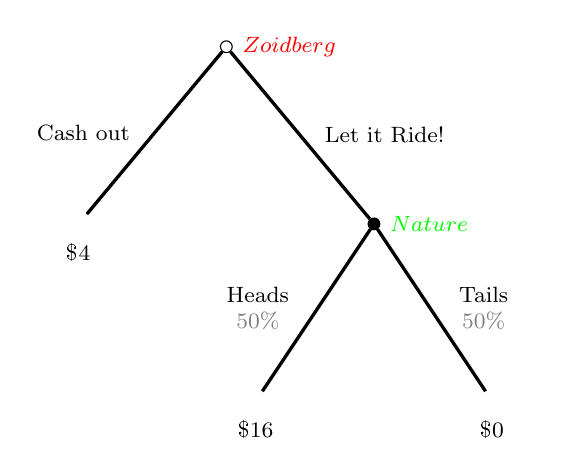
\begin{tikzpicture}[scale=1.5,font=\footnotesize, edge from parent/.style={draw, very thick}]
      \tikzstyle{solid node}=[circle,draw,inner sep=1.5,fill=black]
      \tikzstyle{hollow node}=[circle,draw,inner sep=1.5]
      \tikzstyle{level 1}=[level distance=15mm,sibling distance=2.5cm]
      \tikzstyle{level 2}=[level distance=15mm,sibling distance=2.0cm]
      \tikzstyle{level 3}=[level distance=15mm,sibling distance=1cm]
      
      \node(0)[hollow node,label=right:{\color{red} $Zoidberg$}]{}
          child{node(1)[label=below:{\$$4$}]{}
              edge from parent node[left,xshift=-5]{Cash out}
          }
          child{node(2)[solid node,label=right:{\color{green}$Nature$}]{}
              child{node[label=below:{\$$16$}]{} edge from parent node[left]{
              \begin{tabular}{c}
                   Heads \\
                   {\color{gray} $50\%$} \\
              \end{tabular}
              }}
              child{node[label=below:{\$$0$}]{} edge from parent node[right]{
              \begin{tabular}{c}
                   Tails \\
                   {\color{gray} $50\%$} \\
              \end{tabular}
              }}
              edge from parent node[right,xshift=5]{Let it Ride!}
          };
    \end{tikzpicture}
  \end{center}
  What is Zoidberg's \textbf{expected value} of \textit{Let it Ride}?
\end{frame}

% - - - - - - - - - - - - - - - - - - - - - - - - - - - - - - - - - - - - - - -

\begin{frame}{Playing with Chance}
  What if the coin is \textit{unfair}?
  \begin{center}
    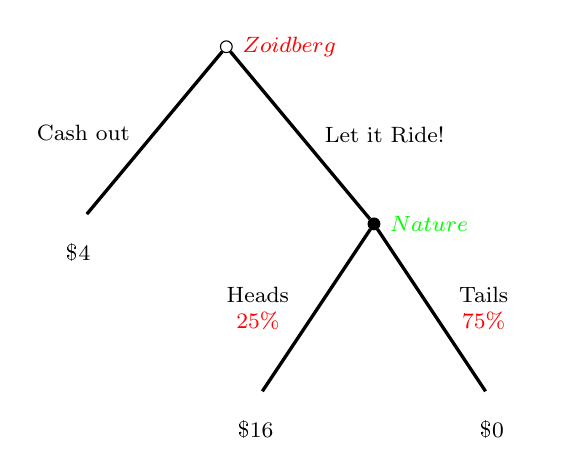
\begin{tikzpicture}[scale=1.5,font=\footnotesize, edge from parent/.style={draw, very thick}]
      \tikzstyle{solid node}=[circle,draw,inner sep=1.5,fill=black]
      \tikzstyle{hollow node}=[circle,draw,inner sep=1.5]
      \tikzstyle{level 1}=[level distance=15mm,sibling distance=2.5cm]
      \tikzstyle{level 2}=[level distance=15mm,sibling distance=2.0cm]
      \tikzstyle{level 3}=[level distance=15mm,sibling distance=1cm]
      
      \node(0)[hollow node,label=right:{\color{red} $Zoidberg$}]{}
          child{node(1)[label=below:{\$$4$}]{}
              edge from parent node[left,xshift=-5]{Cash out}
          }
          child{node(2)[solid node,label=right:{\color{green}$Nature$}]{}
              child{node[label=below:{\$$16$}]{} edge from parent node[left]{
              \begin{tabular}{c}
                   Heads \\
                   {\color{red} $25\%$} \\
              \end{tabular}
              }}
              child{node[label=below:{\$$0$}]{} edge from parent node[right]{
              \begin{tabular}{c}
                   Tails \\
                   {\color{red} $75\%$} \\
              \end{tabular}
              }}
              edge from parent node[right,xshift=5]{Let it Ride!}
          };
    \end{tikzpicture}
  \end{center}  
  What is the \textbf{expected value} now? \\ 
  Should {\color{red} Zoidberg} take the gamble?
\end{frame}

% - - - - - - - - - - - - - - - - - - - - - - - - - - - - - - - - - - - - - - -

\begin{frame}{Risk Preferences}
  Is \textbf{expected value} always the same as \alert{expected utility}?
  \begin{itemize}
    \item Suppose that I offered you a different gamble:
    \begin{itemize}
      \item \textbf{Option 1:} You get \$1,000,000 with 50\% chance,
      \$0 with 50\% chance.
      \item \textbf{Option 2:} You get \$400,000 for certain.
    \end{itemize}
    \item Which would you choose?
  \end{itemize}
\end{frame}

% - - - - - - - - - - - - - - - - - - - - - - - - - - - - - - - - - - - - - - -

\begin{frame}{Risk Preferences}
  Why would I prefer \textbf{Option 2} when it gives a lower \textit{expected payout}? 
  \begin{itemize}
    \item \$400,000 is still a life changing amount of money, 
    \item but my \alert{marginal benefit} from going from \$400,000 to \$1,000,000 
    is less than my \alert{marginal benefit} from going from \$0 to \$400,000.
    \item The \textbf{risk} of going home empty handed isn't worth the 
    payout that is a marginally larger life-changing amount of money.
  \end{itemize}
\end{frame}

% - - - - - - - - - - - - - - - - - - - - - - - - - - - - - - - - - - - - - - -

\begin{frame}{Risk Preference: Risk Aversion}
  What would a utility function with \alert{diminishing marginal benefit} 
  look like?
  \vspace{50mm}
\end{frame}

% - - - - - - - - - - - - - - - - - - - - - - - - - - - - - - - - - - - - - - -

\begin{frame}{Playing with Chance: Risk Averse Utility}
  Now suppose that {\color{red} Zoidberg}'s utility is 
  ${\color{red} U_{Z}(\$x) = \sqrt{x}}$
  \begin{center}
    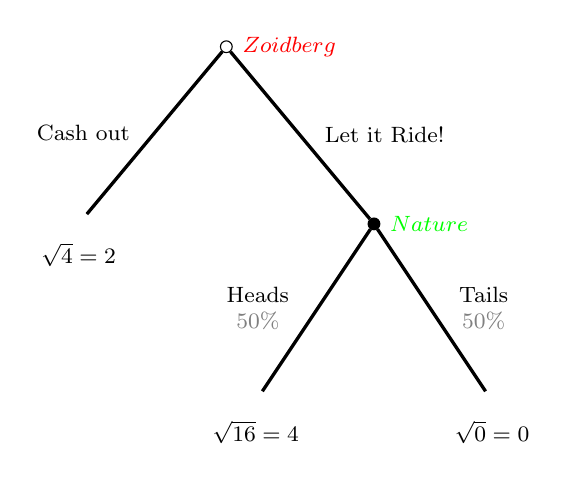
\begin{tikzpicture}[scale=1.5,font=\footnotesize, edge from parent/.style={draw, very thick}]
      \tikzstyle{solid node}=[circle,draw,inner sep=1.5,fill=black]
      \tikzstyle{hollow node}=[circle,draw,inner sep=1.5]
      \tikzstyle{level 1}=[level distance=15mm,sibling distance=2.5cm]
      \tikzstyle{level 2}=[level distance=15mm,sibling distance=2.0cm]
      \tikzstyle{level 3}=[level distance=15mm,sibling distance=1cm]
      
      \node(0)[hollow node,label=right:{\color{red} $Zoidberg$}]{}
          child{node(1)[label=below:{$\sqrt{4} = 2 $ }]{}
              edge from parent node[left,xshift=-5]{Cash out}
          }
          child{node(2)[solid node,label=right:{\color{green}$Nature$}]{}
              child{node[label=below:{$\sqrt{16} = 4$}]{} edge from parent node[left]{
              \begin{tabular}{c}
                   Heads \\
                {\color{gray} $ 50\% $}
              \end{tabular}
              }}
              child{node[label=below:{$\sqrt{0} = 0$}]{} edge from parent node[right]{
              \begin{tabular}{c}
                   Tails \\
                   {\color{gray} $ 50\% $} \\
              \end{tabular}
              }}
              edge from parent node[right,xshift=5]{Let it Ride!}
          };
    \end{tikzpicture}
  \end{center}  
  Would {\color{red} Zoidberg} be willing to cash out?
\end{frame}

% - - - - - - - - - - - - - - - - - - - - - - - - - - - - - - - - - - - - - - -

\begin{frame}{Risk Preference: Risk Seeking}
  What would a utility function with \alert{increasing marginal benefit} 
  look like?
  \vspace{50mm}
\end{frame}

% - - - - - - - - - - - - - - - - - - - - - - - - - - - - - - - - - - - - - - -

\begin{frame}{Playing with Chance: Risk Seeking Utility}
  Now suppose that {\color{blue} Bender}'s utility is 
  ${\color{blue} U_{B}(\$x) = x^2}$
  \begin{center}
    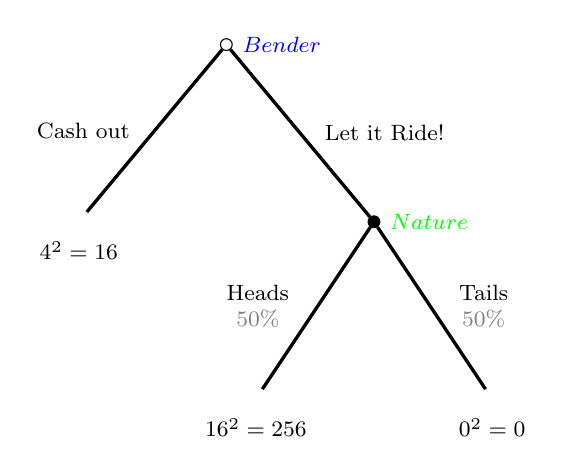
\begin{tikzpicture}[scale=1.5,font=\footnotesize, edge from parent/.style={draw, very thick}]
      \tikzstyle{solid node}=[circle,draw,inner sep=1.5,fill=black]
      \tikzstyle{hollow node}=[circle,draw,inner sep=1.5]
      \tikzstyle{level 1}=[level distance=15mm,sibling distance=2.5cm]
      \tikzstyle{level 2}=[level distance=15mm,sibling distance=2.0cm]
      \tikzstyle{level 3}=[level distance=15mm,sibling distance=1cm]
      
      \node(0)[hollow node,label=right:{\color{blue} $Bender$}]{}
          child{node(1)[label=below:{$4^2 = 16 $ }]{}
              edge from parent node[left,xshift=-5]{Cash out}
          }
          child{node(2)[solid node,label=right:{\color{green}$Nature$}]{}
              child{node[label=below:{$16^2 = 256$}]{} edge from parent node[left]{
              \begin{tabular}{c}
                   Heads \\
                {\color{gray} $ 50\% $}
              \end{tabular}
              }}
              child{node[label=below:{$0^2 = 0$}]{} edge from parent node[right]{
              \begin{tabular}{c}
                   Tails \\
                   {\color{gray} $ 50\% $} \\
              \end{tabular}
              }}
              edge from parent node[right,xshift=5]{Let it Ride!}
          };
    \end{tikzpicture}
  \end{center}  
  Would {\color{blue} Bender} be willing to cash out?
\end{frame}

% - - - - - - - - - - - - - - - - - - - - - - - - - - - - - - - - - - - - - - -

\begin{frame}{Measuring Risk Preferences}
  Both utility functions are \textbf{rational}, 
  but lead to much different behavior. \\
  How can we tell whether someone is 
  \alert{risk averse} or \alert{risk seeking}?
  \pause 
  \begin{itemize}
    \item look at their \alert{revealed preferences} 
    through the choices they make.
  \end{itemize}
\end{frame}

% - - - - - - - - - - - - - - - - - - - - - - - - - - - - - - - - - - - - - - -

\begin{frame}{Measuring Risk Preferences - Certainty Equivalent}
  \begin{itemize}
    \item Suppose that you don't know my risk preference 
    \item but you can offer me a choice between: 
    \begin{itemize}
      \item A \textbf{lottery} $L$ between \$$A$ and \$$B$ with probability $p$
      \item or a \textbf{certain} amount \$$x$ of your choosing. 
    \end{itemize}
    \item The certain amount $x$ that would make me \textit{indifferent}
    between the lottery and taking the sure payment 
    is called the \alert{certainty equivalent} of $L$.
  \end{itemize}
\end{frame}

% - - - - - - - - - - - - - - - - - - - - - - - - - - - - - - - - - - - - - - -

\begin{frame}{Measuring Risk Preferences - Certainty Equivalent}
  \begin{itemize}
    \item If my \textbf{certainty equivalent} 
    is less than the expected value of the lottery 
    \begin{itemize}
      \item you know that I am \alert{risk averse} 
    \end{itemize}
    \item If the \textbf{certainty equivalent} $>$ \textbf{$\mathbb{E}[L]$} 
    \begin{itemize}
      \item I am \alert{risk seeking}
    \end{itemize}
    \item If the \textbf{certainty equivalent} $=$ \textbf{$\mathbb{E}[L]$}
    \begin{itemize}
      \item I am \alert{risk neutral} 
    \end{itemize}
  \end{itemize} 
\end{frame}
